\chapter{SeqZip - Development and Applications} % Main chapter title
\label{Chapter2} 
\lhead{Chapter 2. \emph{SeqZip - Development and Applications}} 
%----------------------------------------------------------------------------------------
\section{SeqZip Overview}\label{sec: SeqZip Overview}
%----------------------------------------------------------------------------------------

Development of the SeqZip methodology began with an attempt to circumvent an obvious shortcoming in second generation HTS\textemdash the short nature of the reads. Until second generation HTS (i.e. reads <100nt on either the Illumina or SOLiD platforms), most sequencing was done using cloned fragments, stored in a bacteria, and analyzed using dideoxy Sanger Sequencing ( see \ref{sec:DNA Sequencing History}. Indeed, this is how most \hyperref[hd:abrevs]{EST}s where analyzed. An extremely powerful feature of these ESTs is that as they represented the sequence of a single clone, from a single original molecule of RNA, the connectivity between sequences that were far apart (>1,000 nt) in the original sequence was maintained. It is this very feature, the continuity of sequence, that allowed whole genome shotgun sequenced to be used, and ESTs to be assembled, into complete genomes, despite sometimes lengthly, and highly repetitive, sretches of DNA (see \ref{sec:DNA Sequencing History}). Once research transitioned over to heavy use of the second generation HTS, all of that connectivity was lost, and all the inherent information with it.

Second generation HTS can be supplemented with other technologies. This has been demonstrated perhaps most successfully with long-read assisted genome assembly \citep{Koren2012a}. Why not supplemental the disconnected nature of short reads with another technilogy? To that end, Phillip Zamore proposed an RNA-templated DNA to DNA ligation approach as drawn in Figure \ref{fig:Original SeqZip Diagram} (see also US Patent application \href{http://1.usa.gov/PTG9BB}{12/906,678}). Using this approach, 2 or more distant sequences of RNA are investigated using short DNA oligonucleotides that hybridize to target sequences, forcing the intervening sequences to loop out. Incorporation of the hybridized DNA via ligation with those of DNAs adjacently hybridized generates a positive read out of sequence presence.

%% ############# FIGURE
\begin{figure}[htbp]
	\centering 
	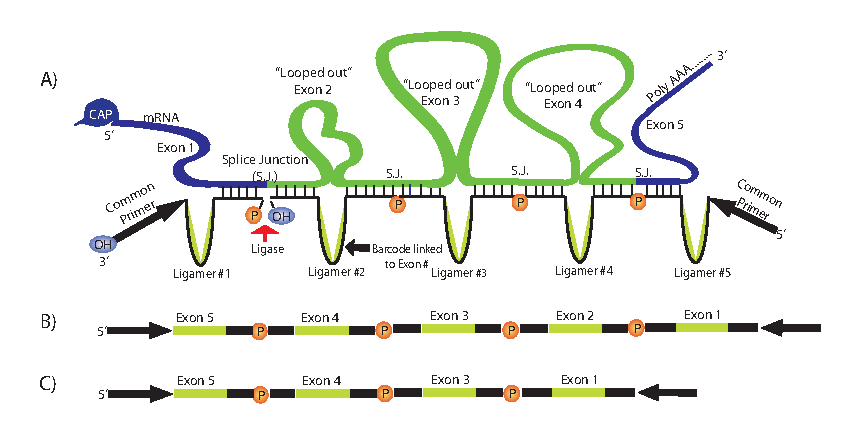
\includegraphics{Figures/Chapter2/OriginalSeqZipDiagram.eps}
	\caption[Original SeqZip Diagram]
	{
		Original SeqZip Diagram\\
		This is the original concept diagram of the SeqZip methodology. (A) Specific DNA oligos target an mRNA and loop out the RNA sequence. Ligases is added to join the DNA oligos together; (B) \& (C) Two different possibilities of ligation products templated from the RNA in (A), where Exon 2 is an cassette exon.
	}
	\label{fig:Original SeqZip Diagram}
\end{figure}
%% ############# FIGURE

Along with Patent \href{http://1.usa.gov/PTG9BB}{12/906,678}, Chapter \ref{Chapter3} presents much of the early and important developmental work demonstrating reduction to practice of this method (termed ``SeqZip"), and its application to investgating connectivity of sequence content in biologically-interesting genes \fn{} and \dscam{}. 

Presented in this Chapter are experiences demonstrating SeqZip application to the following questions and issues:
\begin{itemize}
	\item Section \ref{sec: Multiplex Gene Study}: Investgation of 10 genes, simultaneously ("Multiplex") for connected AS decisions
	\item Section \ref{sec: SeqZip Intergrity}: Using SeqZip to investigate the interigy of RNA molecules
 	\item Section \ref{sec: precursor TX}: Using SeqZip to demonstrate the presence of long, continuous piRNA precusors
\end{itemize}

The three sections contrast with Chapter \ref{Chapter3} in some important ways. First, Section \ref{sec: Multiplex Gene Study} demonstrates that the SeqZip method can not only be used to investigate one, extremely complex Alternatively splice gene, such as \dscam{} in a c comprehensive manner, but can also be applied to looking at multiple genes at once. Seciton \ref{sec: SeqZip Intergrity} expoits an important subtle feature of the method\textemdash that the RNA must be intact in order to produce a ligation product. This can be used to report on a fraction of RNA that is intact, and deduce meaningful information such as the amount of RNA virus that is intact (see \ref{subsec: HIV}), or the existance of as-yet unobserved mega transcripts, like mammalian piRNA precursors (see \ref{sec: precursor TX} and \citep{Li2013h,Li2013}).

%----------------------------------------------------------------------------------------
\section{Multiplex Gene Study}\label{sec: Multiplex Gene Study}
%----------------------------------------------------------------------------------------

Is the coordination discussed in section \ref{sec: Coordination in splicing} a general phenomenon? One of the major goals of developing the SeqZip methodology was investigating potential coordination genome-wide. By genome-wide, what we really mean is to analyze many (or all) of the RNA transcripts in a tissue for evidence of coordinated splicing decisions. When development of the method reached the point that it could be applied in a multiplex study, I did not posses the bioinformatic skills necessary to 1) design ligamers in an automated and high-throughput fashion and 2) identify target transcripts, exons, and sequences to investigate for potential connectivity. Both of these points are discussed later(see \ref{AppendixC}\ref{Chapter5}. 

In order to make some progress on applying the technique to multiple genes at once, I used data presented by \citet{Fagnani2007}. This paper identified genes displaying tissue-specific splicing patterns, focusing on those with CNS-specific patterns. Once section focused on ``''Coordination between AS events belonging to the same genes,'' and seemed to be the exact type of data we were interested in applying the SeqZip method too. Five hundred of the 3,044 genes investigated by their microarrays contained 2\textendash 5 alternative exons. \citet{Fagnani2007} contained an additional data file listing all pair-wise combinations of alternative exons in the same gene (with that gene having significant expression in >20 different tissues), along with the standard and partial spearman correlations. 

It is important to note that the genes above also contain alternative first exons, a prominant type of AS (see figure \ref{fig:asEventsBarChart}). Indeed, from microarrays studies, it has been estimated that approximately 16\%\textendash 23\% of all AS events involve alternative first and last exons \citep{Bingham2008a}. It is known that, through alternative use of first and last exons, cells can fine-tune a transcript’s untranslated region (UTR) and control many aspects of mRNA regulation including nuclear export, localization, expression, and stability \citep{Hughes2006}. In support of the importance of alternative UTRs in tuning of gene expression, a landmark RNA-Seq study demonstrated a high occurrence of alternative first and last exon splicing, with alternative tandem 3\textprime~ UTR usage being the most highly tissue-dependent form of AS observed \citep{Wang2008}. The current model of spatial proximity between 5\textprime~ and 3\textprime~ UTRs is suggestive of their possible interdependence. In our multiplez analysis, we included genes potentially displaying interdependence between first and last exons. Discovery of interdependence would lead to many questions into how specific combinations of UTRs can influence mRNA processing downstream of AS.

Using the \citet{Fagnani2007} data, I filtered exon pairs to those with a distance >350 nt in the final pre-mRNA. I also visualized their transcript achetecture, and EST evidence using NCBIs AceView tool \citep{Thierry-Mieg2006}. For example, the exons with strong correlation of expression in \textit{Chl1} are in the beginning (second exon) and end (fourth from last exon, accession BC060216) with plenty of supporting evidence for these exons being expressed and skipped. After combing through \citep{Fagnani2007} data for a group of about 10 genes. The genes examined are presented in Table \ref{table: BigSpanGenes}.

% !TEX root = /Users/royc/Google_Drive/Thesis/RoyC_Umass_Thesis.tex
\begin{table}[h]\small
  \begin{tabular}{|l|r|r|r|r|}

  \hline
  \textbf{Gene name} & \textbf{nt mRNA between} & \textbf{possible isoforms} & \textbf{Exon 1} & \textbf{Exon 2} \\ \hline
  Chl1               & 4665                              & 18                         & 2               & 24              \\ \hline
  Mdm1               & 1846                              & 4                          & EDA             & IIICS           \\ \hline
  PTPRF-Y            & 1633                              & 4                          & 2               & 13              \\ \hline
  Cacna1c            & 1403                              & 4                          & 15              & 21/22           \\ \hline
  PTPRF-X            & 936                               & 4                          & 9/10            & 21              \\ \hline
  FN1                & 813                               & 8                          & 13/14           & 21/22           \\ \hline
  Apbb1              & 802                               & 260                        & 1/2b            & 2/3e            \\ \hline
  Agrn               & 736                               & 8                          & 33/34c          & 33/34a          \\ \hline
  Exoc7              & 513                               & 4                          & 7               & 13              \\ \hline
  Prom1              & 512                               & 4                          & 7               & 9               \\ \hline
  Lphn2              & 396                               & 32                         & 19              & 24/25a          \\ \hline
  \end{tabular}
    \caption[Mouse genes with large sequence between suggested coordinated cassette exons]
    {
      A list of 11 genes investigated in section \ref{SeqZipMethod:sec:Multiplex Gene Study}. Coordination between exons first suggested by \citep{Fagnani2007}.
      }
    \label{table: BigSpanGenes}
  \end{table}


I hand-designed ligamers to observe potentially coordinated splicing decisions. These oligos were then ordered from IDT in a 96-well plate format, pooled according to gene, and used to develop a multiplex approach to applying SeqZip, as well as investigate coordination between these exons, in these genes, using mouse total RNA from brains.

%% ############# FIGURE
\begin{figure}[htbp]
	\centering 
	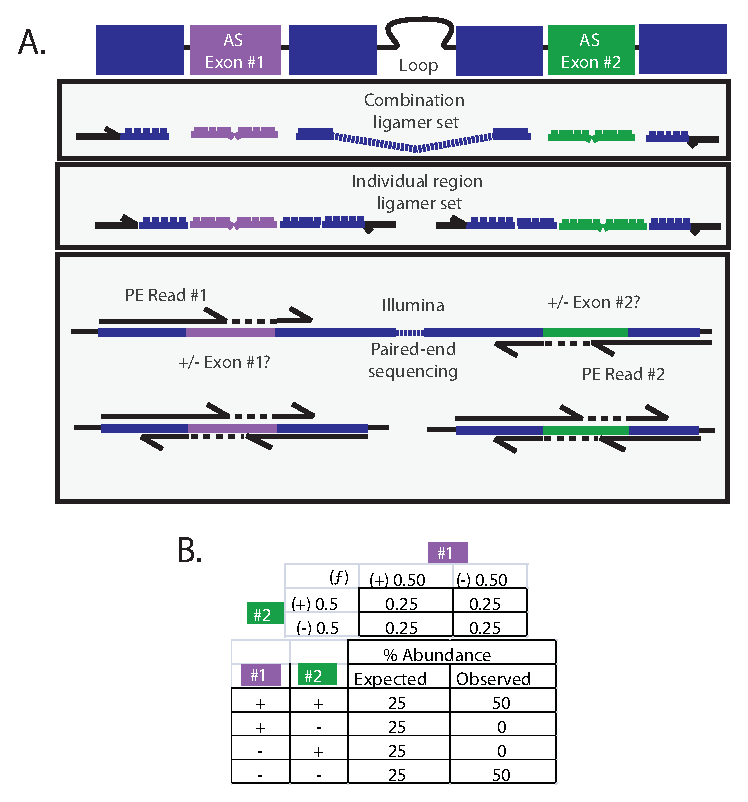
\includegraphics{Figures/Chapter2/10GeneSetSchematic.eps}
	\caption[10 Gene Set schematic]
	{
		10 Gene set schematic\\
		\hl{caption next}
	}
	\label{fig:Original SeqZip Diagram}
\end{figure}
%% ############# FIGURE


%----------------------------------------------------------------------------------------
\section{Determining RNA integrity using SeqZip}\label{sec: SeqZip Intergrity}
%----------------------------------------------------------------------------------------

%-----------------------------------
\subsection{Demonstration of Concept}
%-----------------------------------

%% ############# FIGURE
\begin{figure}[htbp]
	\centering 
	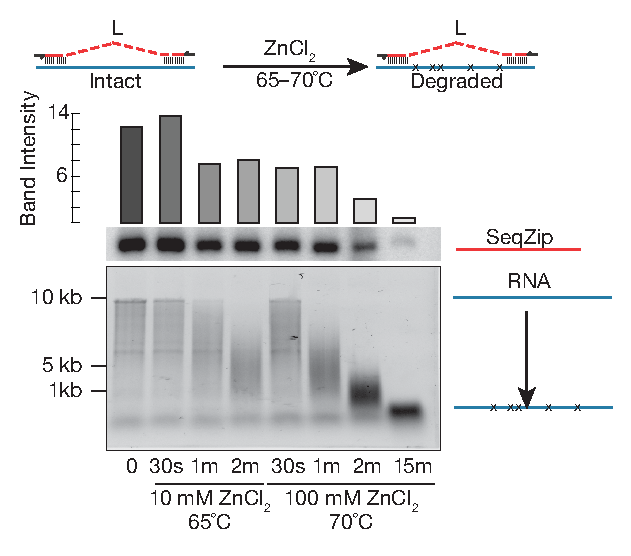
\includegraphics{Figures/Chapter2/DegreadedRNABySeqZip.eps}
	\caption[Ligation product tied to RNA integrity]
	{
		Ligation product tied to RNA integrity\\
		\hl{figure Caption}
	}
	\label{fig:Ligation product and RNA integrity}
\end{figure}
%% ############# FIGURE

\lipsum[1-3]

%% ############# FIGURE
\begin{figure}[htbp]
	\centering 
	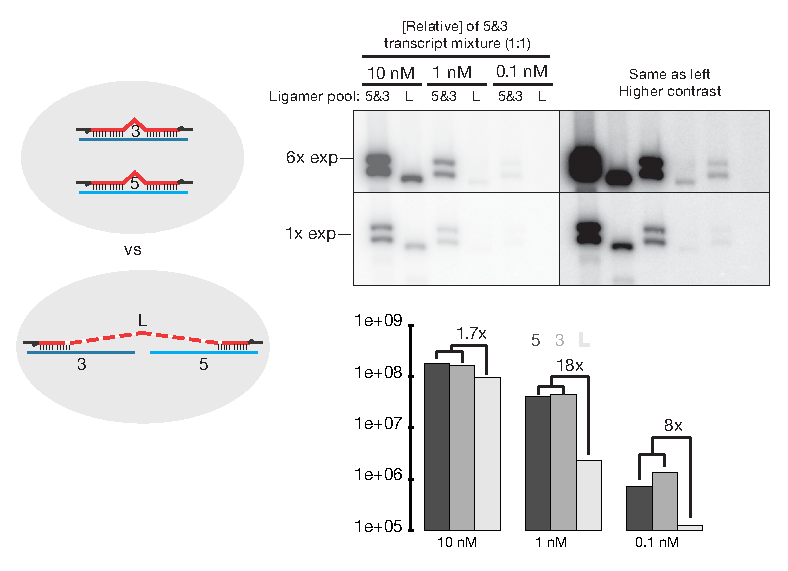
\includegraphics{Figures/Chapter2/TransRNAWithSeqZip.eps}
	\caption[Trans Transcript investigation]
	{
		Trans Transcript investigation\\
		\hl{figure Caption}
	}
	\label{fig:Ligation product and RNA integrity}
\end{figure}
%% ############# FIGURE

%-----------------------------------
\subsection{Investigating HIV viral genome integrity using SeqZip}\label{subsec: HIV}
%-----------------------------------


%! Base the discussion off the introduction in the HIV paper (Serquiña et al. 2013)

MOV10L1 is implicated in HIV genome stability and intactness. We sought to measure the effects of a point mutant in the ATPase domain of MOV10L1 on the ‘intactness’ of the HIV genome. Viral particles contain two copies of the ssRNA HIV genome. Proteomics studies have measured MOV10L1 and Upf1 in viral particles, implicated these proteins, which are known helicases, in the maintained and infectivity of HIV.

%-----------------------------------
\subsection{Design of HIV ligamers}
%-----------------------------------

Research into the integrity of the HIV RNA genome using SeqZip began with designing a set of ligamers against two different clones. The first clone, targeting transcripts from the M19921 plasmid (so called ``M'' clone), and transcripts from the K03455 clone contain nearly identical sequences with respect to the genome itself, and differ mostly in plasmid originating sequences. We targeted a difference in sequence for one site of ligation (Fig3-11A). Three different pools of ligamers were created initially: a Five(5) ligamer pool, with three ligamers design to test for the presence of sequence in the first 1,140 nt of the HIV genome, importantly the first site of ligation in the 5 region pool should contain a mismatch in the K clone sequence; a three(3) pool, testing the last 1,210 nt of the genome, and a Long (L) ligamer pool, also containing three ligamers, but the middle ligamer of which would span the 5 and 3 regions, looping out 8,633 nt of sequence in the middle of the HIV genome. In vitro transcripts were created using both the K and M clone plasmids. These transcripts were added to a background of total MEF RNA, and the SeqZIp assay was performed. Ligation products were successfully amplified from all ligamer pools when using the M clone transcript and all three ligamer pools. Also the abundance of these ligation products, as measured by endpoint PCR, seemed to be spike-concentration dependent. Notably, Ligation products were not obtained from the K clone using either the 5 or L ligamer pools, likely due to the mismatch between the transcript and the ligamers at the site of ligation. Also of note was the appearance of ligation products from purified endogenous virons of the M clone from all three ligamer pools, and the absence of products from virions purified from plasmids containing a defective protein, Gag, essential for viral packaging. 

%% ############# FIGURE
\begin{figure}[htbp]
	\centering 
	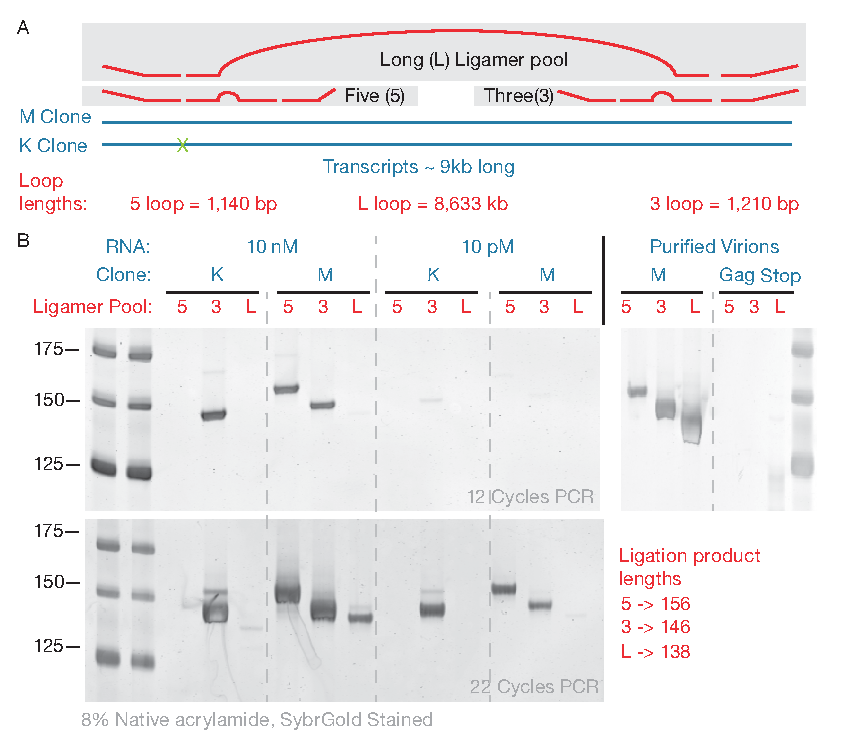
\includegraphics{Figures/Chapter2/HIVviaSeqZip.eps}
	\caption[SeqZip can examine HIV transcript integrity]
	{
		SeqZip can examine HIV transcript integrity\\
		\hl{figure Caption}
	}
	\label{fig:Hiv tx via SeqZip}
\end{figure}
%% ############# FIGURE

%----------------------------------------------------------------------------------------
\section{Continuity of piRNA precursor transcripts}\label{sec: precursor TX}
%----------------------------------------------------------------------------------------

%% ############# FIGURE
\begin{figure}[htbp]
	\centering 
	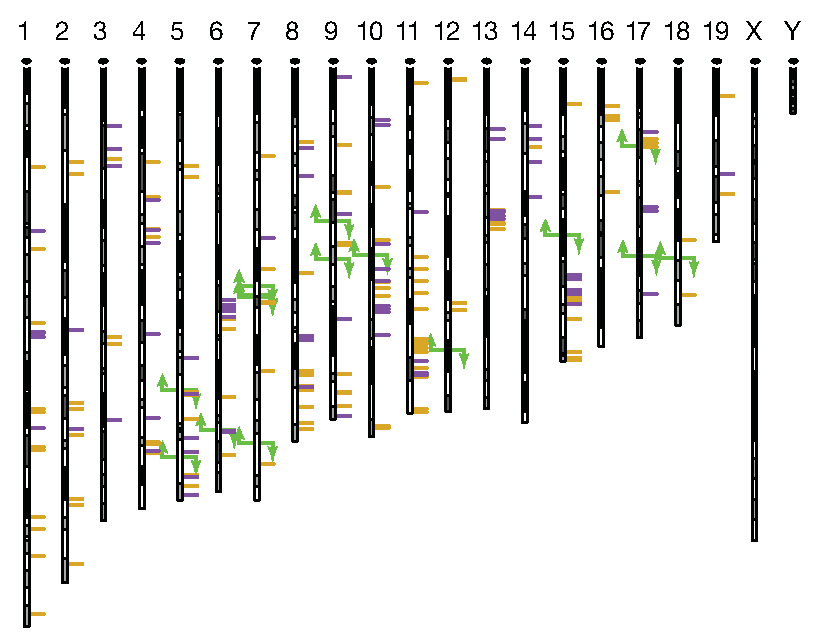
\includegraphics{Figures/Chapter2/PrecursorLocations.eps}
	\caption[piRNA precursor locations]
	{
		piRNA precursor locations\\
		\hl{figure Caption}
	}
	\label{fig:Hiv tx via SeqZip}
\end{figure}
%% ############# FIGURE


%Table 3 1, Just 9 clusters from 5 promoters generate >50% of 14.5 dpp (pachytene) piRNAs
\begin{table}[h]\small
\begin{tabular}{llrrr}
\hline
\textbf{Cluster Name} & \textbf{\begin{tabular}[c]{@{}c@{}}Matched \\ Cluster\end{tabular}} & \textbf{\begin{tabular}[c]{@{}c@{}}Unique-mapping \\ piRNAs @ \\ wt.14dpp\end{tabular}} & \textbf{\begin{tabular}[c]{@{}c@{}}Fraction of \\ pachytene \\ piRNAs\end{tabular}} & \textbf{\begin{tabular}[c]{@{}c@{}}Cumulative\\  pachytene\\  piRNAs\end{tabular}} \\ \hline
17-qA3.3-26735.1      & 17-qA3.3-27363                                                      & 3,021,022                                                                               & 17.2                                                                                & 17.2                                                                               \\
17-qA3.3-27363.1      & 17-qA3.3-26735                                                      & 1,742,695                                                                               & 9.9                                                                                 & 27.2                                                                               \\
9-qC-31469.1          & 9-qC-10667                                                          & 1,006,333                                                                               & 5.7                                                                                 & 32.9                                                                               \\
9-qC-10667.1          & 9-qC-31469                                                          & 272,385                                                                                 & 1.6                                                                                 & 34.5                                                                               \\
7-qD2-24830.1         & 7-qD2-11976                                                         & 652,564                                                                                 & 3.7                                                                                 & 38.2                                                                               \\
7-qD2-11976.1         & 7-qD2-24830                                                         & 280,312                                                                                 & 1.6                                                                                 & 39.8                                                                               \\
6-qF3-28913.1         & 6-qF3-8009                                                          & 564,930                                                                                 & 3.2                                                                                 & 43.0                                                                               \\
6-qF3-8009.1          & 6-qF3-28913                                                         & 180,210                                                                                 & 1.0                                                                                 & 44.0                                                                               \\
2-qE1-35981.1         & NA                                                                  & 1121042                                                                                 & 6.4                                                                                 & 50.4                                                                               \\ \hline
\end{tabular}
  \caption[Just 9 piRNA genes create >50\% of mammalian piRNAs]{\hl{caption}}
  \label{tab:FlyGenesWithManyTx}
\end{table}

%% ############# FIGURE
\begin{figure}[htbp]
	\centering 
	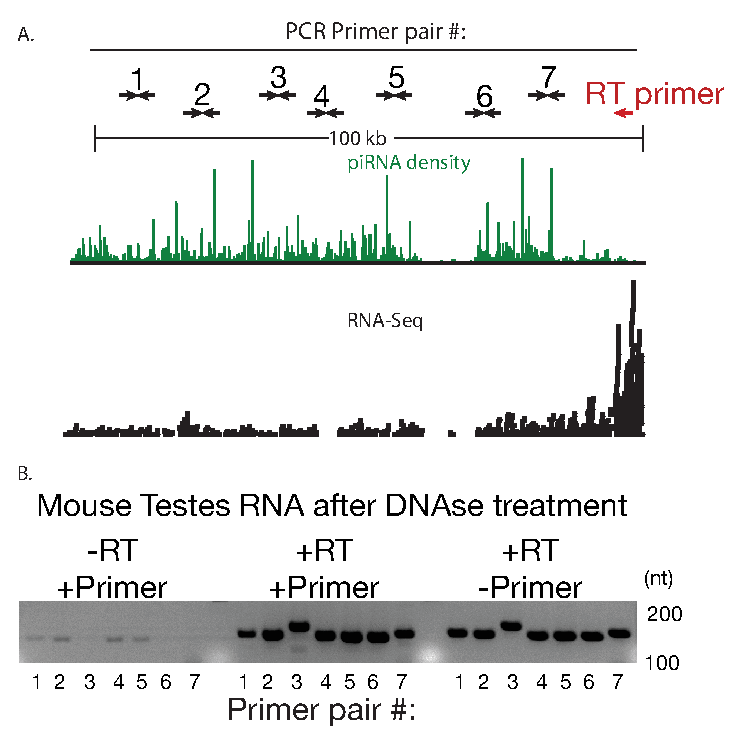
\includegraphics{Figures/Chapter2/RTDoesntWork.eps}
	\caption[pRT Doesn't Work for piRNA precursors]
	{
		RT Doesn't Work for piRNA precursors\\
		\hl{figure Caption}
	}
	\label{fig:Hiv tx via SeqZip}
\end{figure}
%% ############# FIGURE

%% ############# FIGURE
\begin{figure}[htbp]
	\centering 
	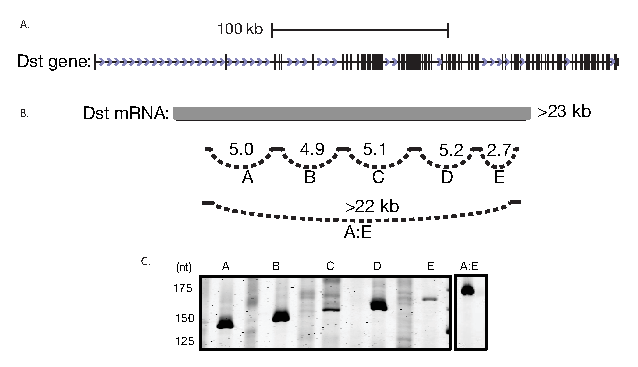
\includegraphics{Figures/Chapter2/dst1.eps}
	\caption[Dst1 by SeqZip]
	{
		Dst1 by SeqZip\\
		\hl{figure Caption}
	}
	\label{fig:Hiv tx via SeqZip}
\end{figure}
%% ############# FIGURE

%% ############# FIGURE
\begin{figure}[htbp]
	\centering 
	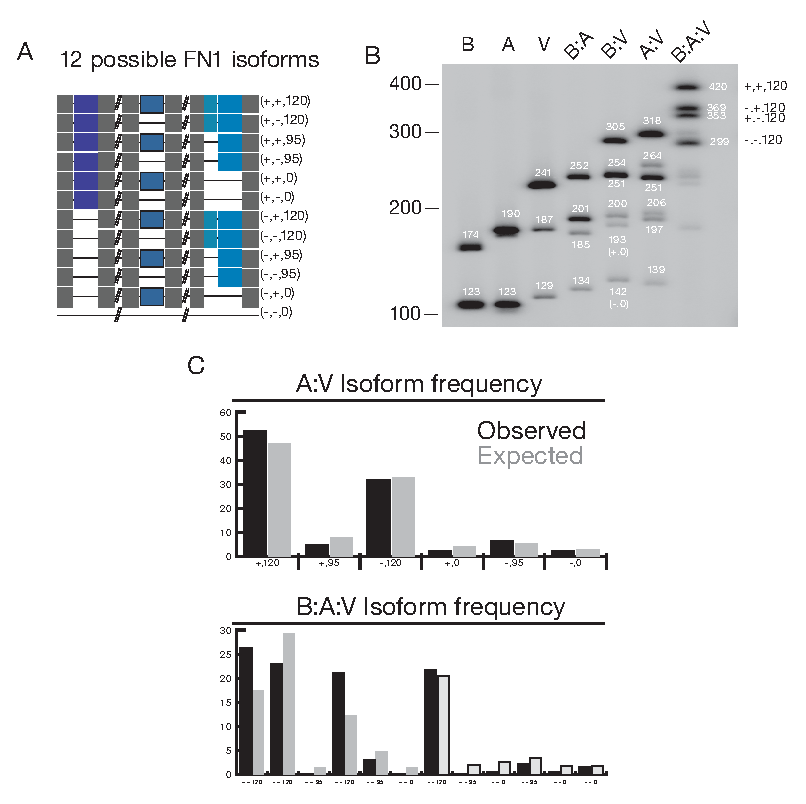
\includegraphics{Figures/Chapter2/fn1ThreeSite.eps}
	\caption[Three sites of AS in \fn{} by SeqZip]
	{
		Capturing AS at three sites and >2kb of mRNA\\
		\hl{figure Caption}
	}
	\label{fig:Hiv tx via SeqZip}
\end{figure}
%% ############# FIGURE

%% ############# FIGURE
\begin{figure}[htbp]
	\centering 
	\includegraphics{Figures/Chapter2/testesSpecificRnaseqPrecursors.eps}
	\caption[Testes Specific RNA precursor expression]
	{
		Testes Specific RNA precursor expression\\
		\hl{figure Caption}
	}
	\label{fig:Hiv tx via SeqZip}
\end{figure}
%% ############# FIGURE


%% ############# FIGURE
\begin{figure}[htbp]
	\centering 
	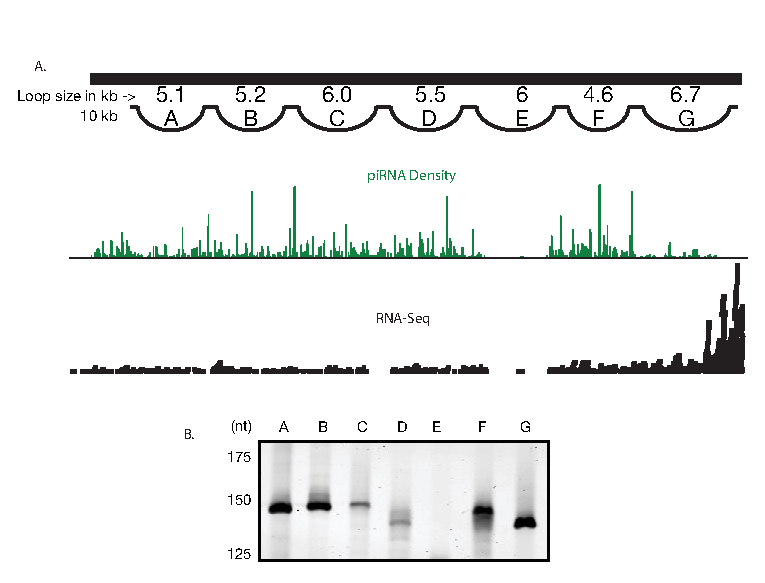
\includegraphics{Figures/Chapter2/piRNAPrecurserAnalyisBySeqZip.eps}
	\caption[piRNA precursor analysis via SeqZip]
	{
		piRNA precursor analysis via SeqZip\\
		\hl{figure Caption}
	}
	\label{fig:Hiv tx via SeqZip}
\end{figure}
%% ############# FIGURE


